\providecommand{\setflag}{\newif \ifwhole \wholefalse}
\setflag
\ifwhole\else

% Typography and geometry ----------------------------------------------------
\documentclass[letterpaper]{scrbook}
\usepackage[inner=3cm,top=2.5cm,outer=3.5cm]{geometry}

\renewcommand\familydefault{bch}
\usepackage[utf8]{inputenc}
\usepackage{microtype}
\usepackage[small]{caption}
\usepackage[small]{titlesec}
\raggedbottom

% Graphics -------------------------------------------------------------------
\usepackage[pdftex]{graphicx}
\graphicspath{{_include/}}
\DeclareGraphicsExtensions{.png,.pdf}

% Code formatting ------------------------------------------------------------
\usepackage{fancyvrb}
\usepackage{courier}
\usepackage{listings}
\usepackage{color}
\usepackage{alltt}


\definecolor{comment}{rgb}{0.60, 0.60, 0.53}
\definecolor{background}{rgb}{0.97, 0.97, 1.00}
\definecolor{string}{rgb}{0.863, 0.066, 0.266}
\definecolor{number}{rgb}{0.0, 0.6, 0.6}
\definecolor{variable}{rgb}{0.00, 0.52, 0.70}
\lstset{
  basicstyle=\ttfamily,
  keywordstyle=\bfseries, 
  identifierstyle=,  
  commentstyle=\color{comment} \emph,
  stringstyle=\color{string},
  showstringspaces=false,
  columns = fullflexible,
  backgroundcolor=\color{background},
  mathescape = true,
  escapeinside=&&,
  fancyvrb
}
\newcommand{\code}[1]{\lstinline!#1!}
\newcommand{\f}[1]{\lstinline!#1()!}



% Links ----------------------------------------------------------------------

\usepackage{hyperref}
\definecolor{slateblue}{rgb}{0.07,0.07,0.488}
\hypersetup{colorlinks=true,linkcolor=slateblue,anchorcolor=slateblue,citecolor=slateblue,filecolor=slateblue,urlcolor=slateblue,bookmarksnumbered=true,pdfview=FitB}
\usepackage{url}

% Tables ---------------------------------------------------------------------
\usepackage{longtable}
\usepackage{booktabs}

% Miscellaneous --------------------------------------------------------------
\usepackage{pdfsync}
\usepackage{appendix}

\usepackage[round,sort&compress,sectionbib]{natbib}
\bibliographystyle{plainnat}


\title{ggplot2}
\author{Hadley Wickham}

\begin{document}
\fi


% SET_DEFAULTS
%   GG-WIDTH: 4  GG-HEIGHT: 4
%   TEX-WIDTH: 0.33\linewidth
%   INLINE: FALSE
%   CACHE: TRUE
% 

% END

\chapter{Polishing your plots for publication}
\label{cha:polishing}

In this chapter you will learn how to prepare polished plots for publication.  Most of this chapter focusses on the theming capability of \ggplot which allows you to control many non-data aspects of plot appearance, but you will also learn how to adjust geom, stat and scale defaults, and the best way to save plots for inclusion into other software packages.  Together with the next chapter, manipulating plot rendering with \code{grid}, you will learn how to control every visual aspect of the plot to get exactly the appearance that you want. \index{Publication!polishing plots for}

The visual appearance of the plot is determined by both data and non-data related components.  Section~\ref{sec:themes} introduces the theme system which controls all aspects of non-data display.  By now you should be familiar with the many ways that you can alter the data-related components of the plot---layers and scales---to visualise your data and change the appearance of the plot.  In Section~\ref{sec:theme-scale-geom} you will learn how you can change the defaults for these, so that you do not need to repeat the same parameters again and again.

Section~\ref{sec:saving} discusses the chapter with a discussion about how to get your graphics out of R and into \LaTeX, Word or other presentation or word-processing software.  Section~\ref{sec:grid-layout} concludes with a discussion of how to lay out multiple plots on a single page.

% Need cross-refs here to changing axis, legend and plot titles
% And guide breaks and legends

\section{Themes} 
\label{sec:themes}

The appearance of non-data elements of the plot is controlled by the theme system. The theme system does not affect how the data is rendered by geoms, or how it is transformed by scales. Themes don't change the perceptual properties of the plot, but they do help you make the plot aesthetically pleasing or match existing style guides. Themes give you control over things like the fonts in all parts of the plot: the title, axis labels, axis tick labels, strips, legend labels and legend key labels; and the colour of ticks, grid lines and backgrounds (panel, plot, strip and legend). \index{Themes} \index{Publication!themes}

This separation of control into data and non-data parts is quite different than base and lattice graphics.  In base and lattice graphics, most functions take a large number of arguments that specify both data and non-data appearance, which makes the functions complicated and hard to learn.  \ggplot takes a different approach: when creating the plot you determine how the data is displayed, then {\em after} it has been created you can edit every detail of the rendering, using the theming system.  Some of the effects of changing the theme of a plot are shown in Figure~\ref{fig:themes}.  The two plots show the two themes included by default in \ggplot.

% FIGURE
%  LABEL: themes
%  CAPTION: The effect of changing themes.  (Left) The default grey theme with
%  grey background and white gridlines.  (Right) the alternative black and 
%  white theme with white background and grey gridlines.  Notice how the 
%  bars, data elements, are identical in both plots.
% 
% qplot(rating, data = movies, binwidth = 1)
% last_plot() + theme_bw()
\input{_include/3e0e8ab1bbb5f015a21069b8058cfbfe.tex}
% END

Like many other areas of \ggplot, themes can be controlled on multiple levels from the coarse to fine.  You can:

\begin{itemize}
  \item Use a built-in theme, as described in Section~\ref{sec:built_in}.  This affects every element of the plot in a visually consistent manner.  The default theme uses a grey panel background with white gridlines, while the alternative theme uses a white background with grey gridlines.

  \item Modify a single element of a built-in theme, as described in  Section~\ref{sec:theme_elements}. Each theme is made up of multiple elements. The theme system comes with a number of built-in element rendering functions with a limited set of parameters.  By adjusting these parameters you can control things like text size and colour, background and grid line colours and text orientation.  By combining multiple elements you can create your own theme.
  
  % \item Write a custom element function with grid, as described in Section~\ref{sec:theme_elements}.  This allows you to completely customise the appearance of any element; you are not restricted to a fixed set of drawing options.  

\end{itemize}

\noindent Generally each of these theme settings can be applied globally, to all plots, or locally to a single plot.  How to do this is described in each section.

\subsection{Built-in themes}
\label{sec:built_in}

There are two built-in themes. \index{Themes!built-in} The default, \f{theme_gray}, uses a very light grey background with white gridlines.  This follows from the advice of \citet{tufte:2006,tufte:1990,tufte:2001,tufte:1997} and \citet{brewer:1994,carr:2002,carr:1994,carr:1999}. We can still see the gridlines to aid in the judgement of position \citep{cleveland:1993a}, but they have little visual impact and we can easily ``tune'' them out. The grey background gives the plot a similar colour (in a typographical sense) to the remainder of the text, ensuring that the graphics fit in with the flow of a text without jumping out with a bright white background. Finally, the grey background creates a continuous field of colour which ensures that the plot is perceived as a single visual entity. \indexf{theme_grey}

The other built-in theme, \f{theme_bw}, has a more traditional white background with dark grey gridlines.  Figure~\ref{fig:themes} shows some of the difference between these themes. \index{White background} \index{Themes!white background} \indexf{theme_bw}

Both themes have a single parameter, \code{base_size}, which controls the base font size.  The base font size is the size that the axis titles use: the plot title is 20\% bigger, and the tick and strip labels are 20\% smaller.  If you want to control these sizes separately, you'll need to modify the individual elements as described in the following section.

You can apply themes in two ways:

\begin{itemize}
  \item Globally, affecting all plots when they are drawn: \code{theme_set(theme_grey())} or \code{theme_set(theme_bw())}.  \f{theme_set} returns the previous theme so that you can restore it later if you want. \indexf{theme_set}
  
  \item Locally, for an individual plot:  \code{qplot(...) + theme_grey()}.  A locally applied theme will override the global default. 
\end{itemize}

\noindent The following example shows a few of these combinations:

% INTERWEAVE
% 
% hgram <- qplot(rating, data = movies, binwidth = 1)
% 
% # Themes affect the plot when they are drawn, 
% # not when they are created
% hgram
% previous_theme <- theme_set(theme_bw())
% hgram
% 
% # You can override the theme for a single plot by adding 
% # the theme to the plot. Here we apply the original theme
% hgram + previous_theme
% 
% # Permanently restore the original theme
% theme_set(previous_theme)
\input{_include/cd885e35f4c994dfea232942468baebb.tex}
% END

\subsection{Theme elements and element functions}
\label{sec:theme_elements}

A theme is made up of multiple \emph{elements} which control the appearance of a single item on the plot, as listed in Table~\ref{tbl:elements}. There are three elements that have individual \code{x} and \code{y} settings: \code{axis.text}, \code{axis.title} and \code{strip.text}. Having a different setting for the horizontal and vertical elements allows you to control how text should appear in different orientations. The appearance of each element is controlled by an \emph{element function}. \index{Themes!elements}

\begin{table}
  \begin{center}
  \begin{tabular}{lll}\\
    \toprule
    Theme element              & Type     & Description  \\
    \midrule                              
    \texttt{axis.line}         & segment  & line along axis  \\
    \texttt{axis.text.x}       & text     & x axis label  \\
    \texttt{axis.text.y}       & text     & y axis label  \\
    \texttt{axis.ticks}        & segment  & axis tick marks  \\
    \texttt{axis.title.x}      & text     & horizontal tick labels  \\
    \texttt{axis.title.y}      & text     & vertical tick labels  \\[0.5em]

    \texttt{legend.background} & rect     & background of legend  \\
    \texttt{legend.key}        & rect     & background underneath legend keys \\
    \texttt{legend.text}       & text     & legend labels  \\
    \texttt{legend.title}      & text     & legend name  \\[0.5em]

    \texttt{panel.background}  & rect     & background of panel  \\
    \texttt{panel.border}      & rect     & border around panel  \\
    \texttt{panel.grid.major}  & line     & major grid lines \\
    \texttt{panel.grid.minor}  & line     & minor grid lines \\
    \texttt{plot.background}   & rect     & background of the entire plot \\
    \texttt{plot.title}        & text     & plot title   \\[0.5em]

    \texttt{strip.background}  & rect     & background of facet labels   \\
    \texttt{strip.text.x}      & text     & text for horizontal strips  \\
    \texttt{strip.text.y}      & text     & text for vertical strips  \\
    \bottomrule                           
  
  \end{tabular}
  \end{center}
  \caption{Theme elements}
  \label{tbl:elements}
\end{table}

There are four basic types of built-in element functions: text, lines and segments, rectangles and blank.  Each element function has a set of parameters that control the appearance as described below:

\begin{itemize}
  \item \f{theme_text} draws labels and headings. You can control the font \code{family}, \code{face}, \code{colour}, \code{size}, \code{hjust}, \code{vjust}, \code{angle} and \code{lineheight}. \index{Themes!labels} \indexf{theme_text}
  
  The following code shows the effect of changing these parameters on the plot title. The results are shown in Figure~\ref{fig:theme-text}. Changing the angle is probably more useful for tick labels.  When changing the angle you will probably also need to change \code{hjust} to 0 or 1.
  
  % FIGLISTING
  %   COL: 3 TEX-WIDTH: 0.33\linewidth GG-WIDTH: 4 GG-HEIGHT: 4
  %   LABEL: theme-text
  %   CAPTION: Changing the appearance of the plot title.
  % 
  % hgramt <- hgram + 
  %   opts(title = "This is a histogram")
  % hgramt
  % hgramt + opts(plot.title = theme_text(size = 20))
  % hgramt + opts(plot.title = theme_text(size = 20, 
  %   colour = "red"))
  % hgramt + opts(plot.title = theme_text(size = 20, 
  %   hjust = 0))
  % hgramt + opts(plot.title = theme_text(size = 20, 
  %   face = "bold"))
  % hgramt + opts(plot.title = theme_text(size = 20, 
  %   angle = 180))
  \input{_include/b1d64f0b186dcd087f3022191fa718ae.tex}  
  % END

  \item \f{theme_line} and \f{theme_segment} draw lines and segments with the same options but in a slightly different way.  Make sure you match the appropriate type or you will get strange grid errors.  For these element functions you can control the \code{colour}, \code{size} and \code{linetype}.  These options are illustrated with the code and the results are shown in Figure~\ref{fig:theme-line}. \indexf{theme_line} \indexf{theme_segment}

  % FIGLISTING
  %   COL: 3 TEX-WIDTH: 0.33\linewidth GG-WIDTH: 4 GG-HEIGHT: 4
  %   LABEL: theme-line
  %   CAPTION: Changing the appearance of lines and segments in the plot.
  % 
  % hgram + opts(panel.grid.major = theme_line(colour = "red"))
  % hgram + opts(panel.grid.major = theme_line(size = 2))
  % hgram + opts(panel.grid.major = theme_line(linetype = "dotted"))
  % hgram + opts(axis.line = theme_segment())
  % hgram + opts(axis.line = theme_segment(colour = "red"))
  % hgram + opts(axis.line = theme_segment(size = 0.5, 
  %   linetype = "dashed"))
  \input{_include/dde612a9ec7c5f9ffa7d96d78efc06db.tex}  
  % END

  \item \f{theme_rect} draws rectangles, mostly used for backgrounds, you can control the \code{fill} colour and border \code{colour}, \code{size} and \code{linetype}.  Examples shown in Figure~\ref{fig:theme-background} are created with the code below: \index{Background} \index{Themes!background} \indexf{theme_rect}
  
  % FIGLISTING
  %   COL: 3 TEX-WIDTH: 0.33\linewidth GG-WIDTH: 4 GG-HEIGHT: 4
  %   LABEL: theme-background
  %   CAPTION: Changing the appearance of the plot and panel background
  % 
  % hgram + opts(plot.background = theme_rect(fill = "grey80", 
  %   colour = NA))
  % hgram + opts(plot.background = theme_rect(size = 2))
  % hgram + opts(plot.background = theme_rect(colour = "red"))
  % hgram + opts(panel.background = theme_rect())
  % hgram + opts(panel.background = theme_rect(colour = NA))
  % hgram + opts(panel.background = 
  %   theme_rect(linetype = "dotted"))
  \input{_include/29fc062ce0fe0eec4383c6d5ce629712.tex}  
  % END

  \item \f{theme_blank} draws nothing.  Use this element type if you don't want anything drawn, and no space allocated for that element.  The following example uses \f{theme_blank} to progressively suppress the appearance of elements we're not interested in. The results are shown in Figure~\ref{fig:theme-blank}.  Notice how the plot automatically reclaims the space previously used by these elements: if you don't want this to happen (perhaps because they need to line up with other plots on the page), use \code{colour = NA, fill = NA} as parameter to create invisible elements that still take up space. \indexf{theme_blank}

  % FIGLISTING
  %   COL: 3 TEX-WIDTH: 0.33\linewidth GG-WIDTH: 4 GG-HEIGHT: 4
  %   LABEL: theme-blank
  %   CAPTION: Progressively removing non-data elements from a plot with 
  %   \f{theme_blank}.
  % 
  % hgramt
  % last_plot() + opts(panel.grid.minor = theme_blank())
  % last_plot() + opts(panel.grid.major = theme_blank())
  % last_plot() + opts(panel.background = theme_blank())
  % last_plot() + 
  %   opts(axis.title.x = theme_blank(), 
  %        axis.title.y = theme_blank())
  % last_plot() + opts(axis.line = theme_segment())
  \input{_include/70ec2776eb18c410c41bdff8cc78807a.tex}  
  % END

\end{itemize}

You can see the settings for the current theme with \f{theme_get}.  The output isn't included here because it takes up several pages.  You can modify the elements locally for a single plot with \f{opts} (as seen above), or globally for all future plots with \f{theme_update}.  Figure~\ref{fig:theme-update} shows the results of pulling together multiple theme settings with the following code. \index{Themes!updating} \indexf{theme_get} \indexf{opts}

% FIGLISTING
%   LABEL: theme-update
%   CAPTION: A bar chart and scatterplot created after a new visually 
%   consistent (if ugly!) theme has been applied.
% 
% old_theme <- theme_update(
%   plot.background = theme_rect(fill = "#3366FF"),
%   panel.background = theme_rect(fill = "#003DF5"),
%   axis.text.x = theme_text(colour = "#CCFF33"),
%   axis.text.y = theme_text(colour = "#CCFF33", hjust = 1),
%   axis.title.x = theme_text(colour = "#CCFF33", face = "bold"),
%   axis.title.y = theme_text(colour = "#CCFF33", face = "bold", 
%    angle = 90)
% )
% qplot(cut, data = diamonds, geom="bar")
% qplot(cty, hwy, data = mpg)
% theme_set(old_theme)
\input{_include/5a2c652b87efb03394169240a1d4635c.tex}
% END

There is some duplication in this example because we have to specify the x and y elements separately.  This is a necessary evil so that you can have total control over the appearance of the elements.  If you are writing your own theme, you would probably want to write a function to minimise this repetition.

% \subsection{Custom element functions}
% \label{sub:custom-elements}
% 
% To see how to write custom element functions, it's good to start by seeing how the built-in element functions work:
% 
% % INTERWEAVE
% % 
% % str(args(theme_text()))
% % str(args(theme_rect()))
% % str(args(theme_line()))
% \input{_include/b9b6e26b5f4fc7e2bb7c9847fb6cd634.tex}
% % END
% 
% You'll notice that these are very similar to the arguments to \f{textGrob}, \f{rectGrob} and \f{polylineGrob} and these are exactly the functions that they are based on.  All that the element function do is set up some defaults.  
% 
% If you want to write your own, you need to copy this basic idea: take position arguments, and return a grid grob.  For example, let's say we'd like to give the strips a 3d appearance.  We can do this by drawing a rectangle, and then drawing highlights on the top-right and low-lights (shadows) on the bottom-left.

\section{Customising scales and geoms}
\label{sec:theme-scale-geom}

When producing a consistent theme, you may also want to tune some of the scale and geom defaults.  Rather than having to manually specify the changes every time you add the scale or geom, you can use the following functions to alter the default settings for scales and geoms. 

\subsection{Scales}
\label{sub:customise-scales}

To change the default scale associated with an aesthetic, use \f{set_default_scale}. (See Table~\ref{tbl:default-scales} for the defaults.)  This function takes three arguments: the name of the aesthetic, the type of variable (discrete or continuous) and the name of the scale to use as the default.  Further arguments override the default parameters of the scale.  The following example sets up colour and fill scales for black-and-white printing: \index{Scales!customising defaults} \indexf{set_default_scale}

% LISTING
% 
% set_default_scale("colour", "discrete", "grey")
% set_default_scale("fill", "discrete", "grey")
% set_default_scale("colour", "continuous", "gradient", 
%   low = "white", high = "black")
% set_default_scale("fill", "continuous", "gradient", 
%   low = "white", high = "black")
\input{_include/ecb0a27ed25fd7ff67db18c3da8bb314.tex}
% END

\subsection{Geoms and stats}
\label{sub:geoms_and_stats}

You can customise geoms and stats in a similar way with \f{update_geom_defaults} and \f{update_stat_defaults}.  Unlike the other theme settings these will only affect plots \emph{created} after the setting has been changed, not all plots drawn after the setting has been changed.  The following example demonstrates changing the default point colour and changing the default histogram to a density (``true'') histogram.  \index{Geoms!customising defaults} \index{Scales!customising defaults} \indexf{update_geom_defaults}

% LISTING
% 
% update_geom_defaults("point", aes(colour = "darkblue"))
% qplot(mpg, wt, data=mtcars)
% update_stat_defaults("bin", aes(y = ..density..))
% qplot(rating, data = movies, geom = "histogram", binwidth = 1)
\input{_include/7510dd49bc3b89dddb8452f6579264f4.tex}
% END

Table~\ref{tbl:geom-defaults} lists all of the common aesthetic defaults.  If you change the defaults for one geom, it's a good idea to change all the defaults for all the other geoms that you commonly use so that your plots look consistent.  If you are unsure on what makes for a valid colour, line type, shape or size, Appendix~\ref{cha:specifications} gives the details. \index{Aesthetics!defaults}

% aes_value <- function(x) paste(names(x), x, sep =": ")
% 
% geoms <- Geom$find_all()
% escape <- function(x) paste("\\code{", x, "}", sep ="")
% aes_defaults <- lapply(geoms, function(y) aes_value(y$default_aes()))
% names(aes_defaults) <- unname(sapply(geoms, function(y) y$objname))
% aes_list <- invert(aes_defaults)
% aes_list <- Filter(function(x) length(x) > 1, aes_list)
% aes_names <- lapply(aes_list, function(x) paste(escape(sort(x)), collapse = ", "))
% names <- colsplit(names(aes_names), ": ", c("aes", "value"))
% names <- apply(names, c(1,2), escape)
% cat(tabulate(data.frame(names, unlist(aes_names))))

\begin{table}
  \begin{center}
  \begin{tabular}{llp{3in}}
    \toprule
    Aesthetic & Default value & Geoms \\
    \midrule
    \code{colour}   & \code{#3366FF}  & \code{contour}, \code{density2d}, \code{quantile}, \code{smooth}                                                                                                                                                                                                                                                                                                                                \\
    \code{colour}   & \code{NA}       & \code{area}, \code{bar}, \code{histogram}, \code{polygon}, \code{rect}, \code{tile}                                                                                                                                                                                                                                                                                                           \\
    \code{colour}   & \code{black}    & \code{abline}, \code{crossbar}, \code{density}, \code{errorbar}, \code{hline}, \code{line}, \code{linerange}, \code{path}, \code{pointrange}, \code{rug}, \code{segment}, \code{step}, \code{text}, \code{vline}                                                                                                                                                                      \\
    \code{colour}   & \code{darkblue} & \code{jitter}, \code{point}                                                                                                                                                                                                                                                                                                                                                                       \\
    \code{colour}   & \code{grey60}   & \code{boxplot}, \code{ribbon}                                                                                                                                                                                                                                                                                                                                                                     \\
    \code{fill}     & \code{NA}       & \code{crossbar}, \code{density}, \code{jitter}, \code{point}, \code{pointrange}                                                                                                                                                                                                                                                                                                                \\
    \code{fill}     & \code{grey20}   & \code{area}, \code{bar}, \code{histogram}, \code{polygon}, \code{rect}, \code{ribbon}, \code{tile}                                                                                                                                                                                                                                                                           \\
    \code{linetype} & \code{1}        & \code{abline}, \code{area}, \code{bar}, \code{contour}, \code{crossbar}, \code{density}, \code{density2d}, \code{errorbar}, \code{histogram}, \code{hline}, \code{line}, \code{linerange}, \code{path}, \code{pointrange}, \code{polygon}, \code{quantile}, \code{rect}, \code{ribbon}, \code{rug}, \code{segment}, \code{smooth}, \code{step}, \code{tile}, \code{vline}   \\
    \code{shape}    & \code{19}       & \code{jitter}, \code{point}, \code{pointrange}                                                                                                                                                                                                                                                                                                                                                   \\
    \code{size}     & \code{0.5}      & \code{abline}, \code{area}, \code{bar}, \code{boxplot}, \code{contour}, \code{crossbar}, \code{density}, \code{density2d}, \code{errorbar}, \code{histogram}, \code{hline}, \code{line}, \code{linerange}, \code{path}, \code{pointrange}, \code{polygon}, \code{quantile}, \code{rect}, \code{ribbon}, \code{rug}, \code{segment}, \code{smooth}, \code{step}, \code{vline}\\
    \code{size}     & \code{2}        & \code{jitter}, \code{point}                                                                                                                                                                                                                                                                                                                                                                       \\
    \code{weight}   & \code{1}        & \code{bar}, \code{boxplot}, \code{contour}, \code{density}, \code{density2d}, \code{histogram}, \code{quantile}, \code{smooth}                                                                                                                                                                                                                                                              \\
 \bottomrule
  \end{tabular}
  \end{center}
  \caption{Default aesthetic values for geoms.  See Appendix~\ref{cha:specifications} for how the values are interpreted by R.}
  \label{tbl:geom-defaults}
\end{table}

\section{Saving your output}
\label{sec:saving}

You have two basic choices of output: raster or vector.  Vector graphics are procedural.  This means that they are essentially ``infinitely'' zoomable; there is no loss of detail.  Raster graphics are stored as an array of pixels and have a fixed optimal viewing size.  Figure~\ref{fig:vector-raster} illustrates the basic differences for a basic circle.  A good description is available at \url{http://tinyurl.com/rstrvctr}. \index{Saving} \index{Exporting} \index{Publication!saving output}

Generally, vector output is more desirable, but for complex graphics containing thousands of graphical objects it can be slow to render.  In this case, it may be better to switch to raster output.  For printed use, a high-resolution (e.g., 600 dpi) graphic may be an acceptable compromise, but may be large. 

\begin{figure}[htbp]
  \centering
    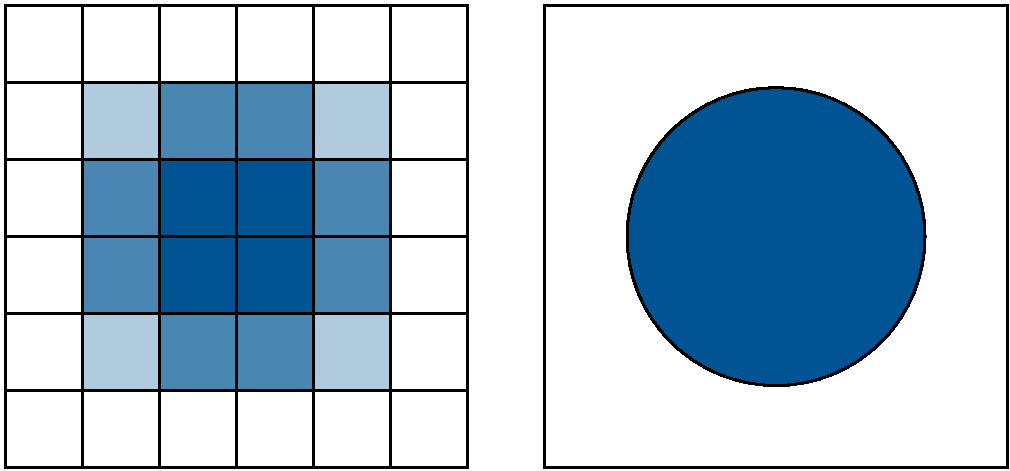
\includegraphics[width= 0.5\linewidth]{vector-raster}
  \caption{The schematic difference between raster (left) and vector (right) graphics. }
  \label{fig:vector-raster}
\end{figure}

To save your output, you can use the typical R way with disk-based graphics devices, which works for all packages, or a special function from \ggplot that saves the current plot: \f{ggsave}. \f{ggsave} is optimised for interactive use and has the following important arguments: \indexf{ggsave}

\begin{itemize}
  \item The \code{path} specifies the path where the image should be saved.  The file extension will be used to automatically select the correct graphics device.
  
  \item Three arguments control output size.  If left blank, the size of the current on-screen graphics device will be used.  \code{width} and \code{height} can be used to specify the absolute size, or \code{scale} to specify the size of the plot relative to the on-screen display.  When creating the final versions of graphics it's a good idea to set \code{width} and \code{height} so you know exactly what size output you're going to get.

  \item For raster graphics, the \code{dpi} argument controls the resolution of the plot. It defaults to 300, which is appropriate for most printers, but you may want to use 600 for particularly high-resolution output, or 72 for on-screen (e.g., web) display.
  
\end{itemize}

The following code shows these two methods. If you want to save multiple plots to a single file, you will need to explicitly open a disk-based graphics device (like \f{png} or \f{pdf}), print the plots and then close it with \f{dev.off}.

% LISTING
% 
% qplot(mpg, wt, data = mtcars)
% ggsave(file = "output.pdf")
% 
% pdf(file = "output.pdf", width = 6, height = 6)
% # If inside a script, you will need to explicitly print() plots
% qplot(mpg, wt, data = mtcars)
% qplot(wt, mpg, data = mtcars)
% dev.off()
\input{_include/dbac803547c6feaaed682c4078eafa18.tex}
% END

Table~\ref{tbl:graphic-recommendation} lists recommended graphic formats for various tasks.  R output generally works best as part of a linux development tool chain: using png or pdf output in \LaTeX{} documents.  With Microsoft Office it is easiest to use a high-resolution (\code{dpi = 600}) png file.  You can use vector output, but neither Windows meta files nor postscript supports transparency, and while postscript prints fine, it is only shown on screen if you add a preview in another software package. Transparency is used to show confidence intervals with the points showing through. If you copy and paste a graph into Word, and see that the confidence interval bands have vanished, that is the cause. The same advice holds for OpenOffice. \index{Exporting!to Word} \index{Exporting!to Powerpoint}

If you are using \LaTeX, I recommend including \verb|\DeclareGraphicsExtensions{.png,.pdf}| in the preamble.  Then you don't need to specify the file extension in \verb|includegraphics| commands, but \LaTeX{} will pick png files in preference to pdf. \index{Exporting!to Latex} I choose this order because you can produce all your files in pdf, and then go back and re-render any big ones as png.  Another useful command is \verb|\graphicspath{{include/}}| which specifies a path in which to look for graphics, allowing you to keep graphics in a separate directory to the text.

\begin{table}
  \begin{center}
  \begin{tabular}{lll}
    \toprule
    Software & Recommended graphics device \\
    \midrule
    Illustrator & svg \\
    latex & ps \\
    MS Office & png (600 dpi) \\
    Open Office & png (600 dpi) \\
    pdflatex & pdf, png (600 dpi) \\
    web & png (72 dpi) \\
    \bottomrule 
  \end{tabular}
  \end{center}
  \caption{Recommended graphic output for different purposes.}
  \label{tbl:graphic-recommendation}
\end{table}

\section{Multiple plots on the same page}
\label{sec:grid-layout}

If you want to arrange multiple plots on a single page, you'll need to learn a little bit of grid, the underlying graphics system used by \ggplot. The key concept you'll need to learn about is a viewport: a rectangular subregion of the display. The default viewport takes up the entire plotting region, and by customising the viewport you can arrange a set of plots in just about any way you can imagine. \index{Layout} \index{Publication!multiple plots on the same page}

To begin, let's create three plots that we can experiment with. When arranging multiple plots on a page, it will usually be easiest to create them, assign them to variables and then plot them. This makes it easier to experiment with plot placement independent of content. The plots created by the code below are shown in Figure~\ref{fig:layout}.

% FIGLISTING
%   LABEL: layout
%   CAPTION: Three simple graphics we'll use to experiment with sophisticated
%   plot layouts.
% 
% (a <- qplot(date, unemploy, data = economics, geom = "line"))
% (b <- qplot(uempmed, unemploy, data = economics) + 
%   geom_smooth(se = F))
% (c <- qplot(uempmed, unemploy, data = economics, geom="path"))
\input{_include/ede394ddaba5b1de12b538d22c060dfe.tex}
% END

\subsection{Subplots}

One common layout is to have a small subplot embedded drawn on top of the main plot.  To achieve this effect, we first plot the main plot, and then draw the subplot in a smaller viewport.  Viewports are created with (surprise!) the \f{viewport} function, with parameters \code{x}, \code{y}, \code{width} and \code{height} to control the size and position of the viewport. By default, the measurements are given in ``npc'' units, which range from 0 to 1. The location (0, 0) is the bottom left, (1, 1) the top right and (0.5, 0.5) the centre of viewport.  If these relative units don't work for your needs, you can also use absolute units, like \code{unit(2, "cm")} or \code{unit(1, "inch")}. \index{Sub-figures} \index{Subplots}

% LISTING 
% 
% # A viewport that takes up the entire plot device
% vp1 <- viewport(width = 1, height = 1, x = 0.5, y = 0.5)
% vp1 <- viewport()
% 
% # A viewport that takes up half the width and half the height, 
% # located in the middle of the plot.
% vp2 <- viewport(width = 0.5, height = 0.5, x = 0.5, y = 0.5)
% vp2 <- viewport(width = 0.5, height = 0.5)
% 
% # A viewport that is 2cm x 3cm located in the center
% vp3 <- viewport(width = unit(2, "cm"), height = unit(3, "cm"))
\input{_include/d68e513659246842e5e046f19b2befde.tex}
% END

By default, the x and y parameters control the location of the centre of the viewport. When positioning the plot in other locations, you may need to use the \code{just} parameter to control which corner of the plot you are positioning.  The following code gives some examples.

% LISTING
% 
% # A viewport in the top right
% vp4 <- viewport(x = 1, y = 1, just = c("top", "right"))
% # Bottom left
% vp5 <- viewport(x = 0, y = 0, just = c("bottom", "right"))
\input{_include/8bc64607ec46dfe26b4255c94c95c5c7.tex}
% END

To draw the plot in our new viewport, we use the \code{vp} argument of the \code{ggplot} \f{print} method.  This method is normally called automatically whenever you evaluate something on the command line, but because we want to customise the viewport, we need to call it ourselves.  The result of this is shown in Figure~\ref{fig:subplot-1}.

% LISTING 
% 
% pdf("polishing-subplot-1.pdf", width = 4, height = 4)
% subvp <- viewport(width = 0.4, height = 0.4, x = 0.75, y = 0.35)
% b
% print(c, vp = subvp)
% dev.off()
\input{_include/748ef3b908f3b3c9c3bb12cff552e776.tex}
% END

This gives us what we want, but we need to make a few tweaks to the appearance: the text should be smaller, we want to remove the axis labels and shrink the plot margins.  The result is shown in Figure~\ref{fig:subplot-2}.

% LISTING
% 
% csmall <- c + 
%   theme_gray(9) + 
%   labs(x = NULL, y = NULL) + 
%   opts(plot.margin = unit(rep(0, 4), "lines"))
% 
% pdf("polishing-subplot-2.pdf", width = 4, height = 4)
% b
% print(csmall, vp = subvp)
% dev.off()
\input{_include/efab9417c676c996c489ec9088c4f6e9.tex}
% END

\begin{figure}[htbp]
  \centering
  \subfigure[Figure with subplot.]{
    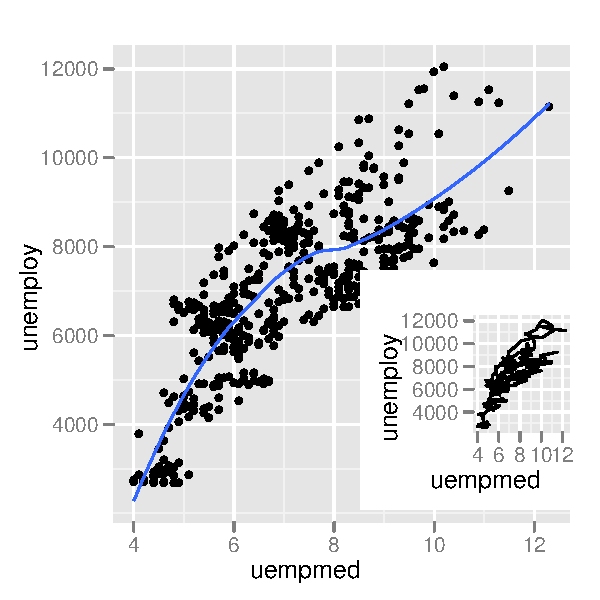
\includegraphics[width=0.5\textwidth]{polishing-subplot-1}
    \label{fig:subplot-1}
  }%
  \subfigure[Subplot tweaked for better display.]{
    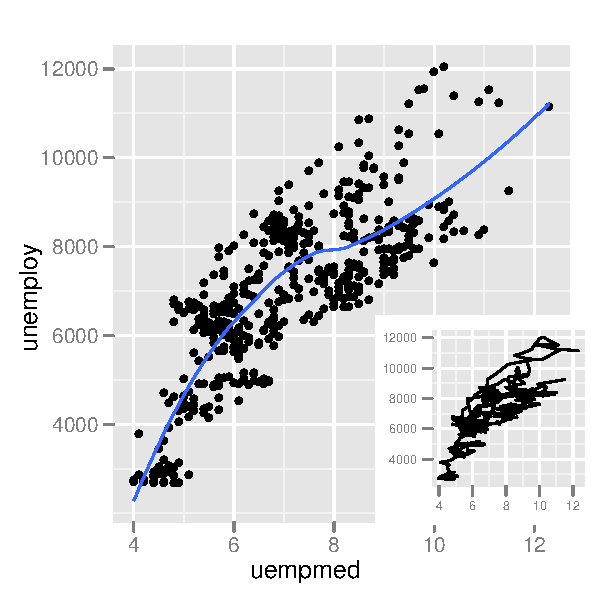
\includegraphics[width=0.5\textwidth]{polishing-subplot-2}
    \label{fig:subplot-2}
  }
  \caption{Two examples of a figure with subplot. It will usually be necessary to tweak the theme settings of the subplot for optimum display.}
  \label{fig:subplot}
\end{figure}

Note we need to use \f{pdf} (or \f{png} etc.) to save the plots to disk because \f{ggsave} only saves a single plot.

\subsection{Rectangular grids} 

A more complicated scenario is when you want to arrange a number of plots in a rectangular grid. Of course you could create a series of viewports and use what you've learned above, but doing all the calculations by hand is cumbersome. A better approach is to use \f{grid.layout}, which sets up a regular grid of viewports with arbitrary heights and widths. You still need to create each viewport, but instead of explicitly specifying the position and size, you can specify the row and column of the layout.

The following example shows how this work.  We first create the layout, here a 2\,$\times$\,2 grid, then assign it to a viewport and push that viewport on to the plotting device.  Now we are ready to draw each plot into its own position on the grid.  We create a small function to save some typing, and then draw each plot in the desired place on the grid.  You can supply a vector of rows or columns to span a plot over multiple cells.  The results are shown in Figure~\ref{fig:layout-2}.

% LISTING
% 
% pdf("polishing-layout.pdf", width = 8, height = 6)
% grid.newpage()
% pushViewport(viewport(layout = grid.layout(2, 2)))
% 
% vplayout <- function(x, y) 
%   viewport(layout.pos.row = x, layout.pos.col = y)
% print(a, vp = vplayout(1, 1:2))
% print(b, vp = vplayout(2, 1))
% print(c, vp = vplayout(2, 2))
% dev.off()
\input{_include/ae7f85b0315e649dcf2d0ab934bacdfa.tex}
% END

\begin{figure}[htbp]
  \centering
    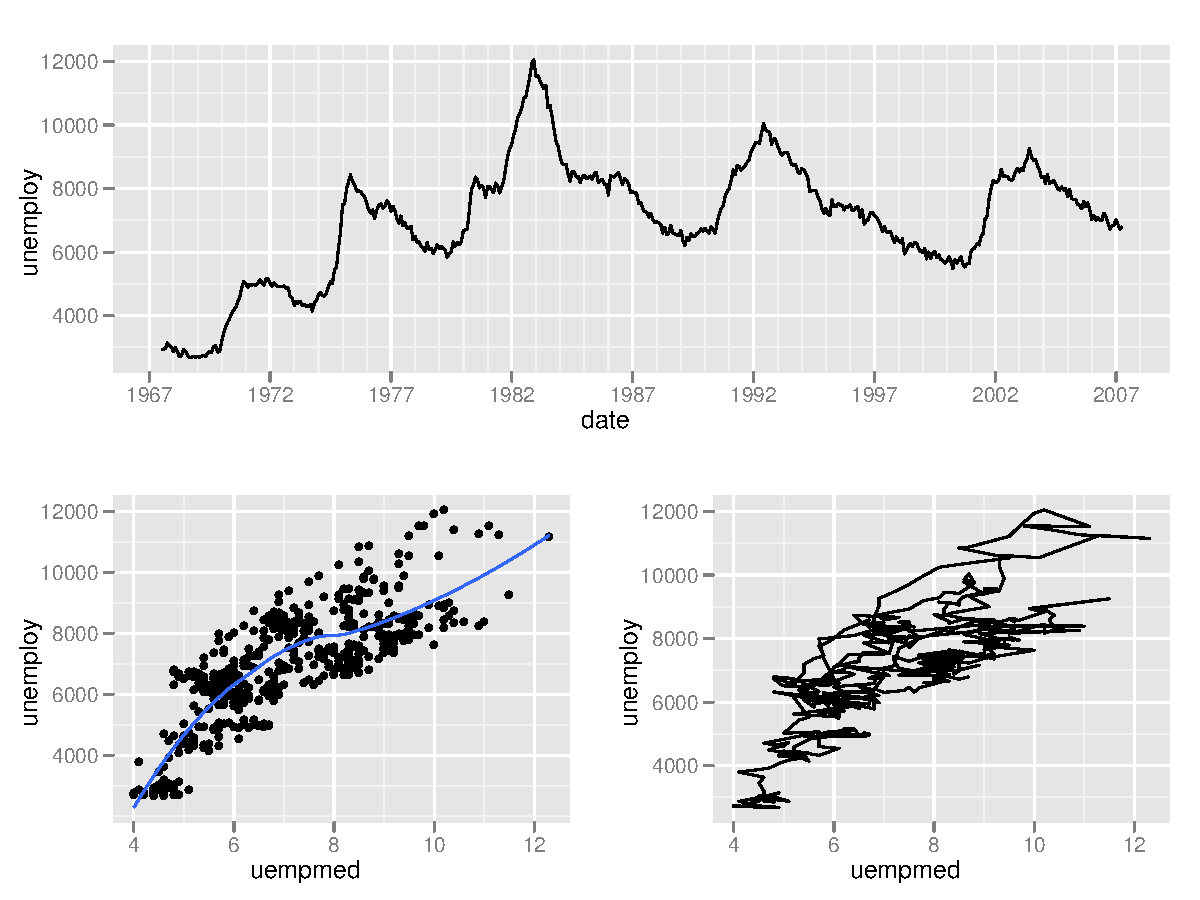
\includegraphics[width=\linewidth]{polishing-layout}
  \caption{Three plots laid out in a grid using \f{grid.layout}.}
  \label{fig:layout-2}
\end{figure}

By default \f{grid.layout} makes each cell the same size, but you can use the \code{widths} and \code{heights} arguments to make them different sizes.  See the documentation for \f{grid.layout} for more examples.

\ifwhole
\else
  \nobibliography{/Users/hadley/documents/phd/references}
  \end{document}
\fi
